\documentclass{/workdir/classes/summary}

\graphicspath{{figures/}}

%タイトルの項目
\title{車椅子卓球の打球精度に寄与する身体動作および筋活動の解析}
\etitle{AnalysisofBodyKinematicsandMuscleActivityContributingtoShotAccuracyinWheelchairTableTennis}
\studentid{03-240351}
\author{明石直也}
\supervisor{山下淳教授}
\abst{
本研究は，個人の身体機能差が著しい車椅子卓球（クラス4）において，打球の正確性を決定づける生体力学的要因を解明することを目的とした．
Chowらが提唱する決定論的モデルを採用し，パフォーマンス（着弾誤差）から，ラケット挙動，関節運動，筋活動へと遡る階層的な解析フレームワークを構築した．
高速度カメラ，モーションキャプチャ，表面筋電図を用いた同期計測実験を行い，機械学習および統計的手法を用いて各階層間の因果関係を分析した．
解析の結果，打球精度を決定づけるラケット要因として「ラケット面角度」「水平打ち出し角」「長軸方向の打点位置」の3点が特定された．
さらに，これらの制御には，運動連鎖に基づく近位（肩・体幹）から遠位（肘・手首）へのエネルギー伝達が不可欠であり，特にインパクトに向けた三角筋前部の活動低下（ブレーキング動作）と，それに伴う遠位セグメントの加速が重要であることを明らかにした．
本研究は，経験則に依存しがちなパラスポーツ指導に対し，客観的データに基づく個別最適化された指導指針を提供するものである．
}

\begin{document}
\maketitle

\section{序論}

\subsection{研究背景}
近年，パラリンピックへの社会的関心の高まりとともにパラスポーツの競技レベルは著しく向上しており，経験則のみならず科学的知見に基づいた指導への需要が急増している．
スポーツバイオメカニクスの分野において，パフォーマンス向上のための指導指針を構築する最も標準的なアプローチは一般化であった．
これは，多数の熟練者の動作データを平均化し，万人に共通する理想的なフォームを導出する手法であり，健常者スポーツにおいては成功を収めてきた\citeen{leesTechniqueAnalysisSports2002}．

一方，パラスポーツにおいては，競技の公平性を担保するために国際パラリンピック委員会（IPC）によるクラス分けが導入されているが\citeen{tweedyInternationalParalympicCommittee2011}，これはあくまで競技上の区分であり，選手間の身体操作の均質性を保証するものではない．実際，Norouziらは車椅子卓球選手において，同一の障害クラス内であっても，脊髄損傷のレベル（完全・不全）の違いによって，打球時の筋活動パターンや発火タイミングに明確な差異が存在することを報告している\cite{norouziElectromyographicAnalysisElite2025}．
このように身体機能の極端な多様性が存在する状況下では，集団の平均モデルを適用することは，各選手が独自に獲得した代償動作や最適化された運動戦略をノイズとして排除することになりかねない．
したがって，パラスポーツの指導現場においては，既存の一般化アプローチには限界があり，各選手固有の残存機能に立脚した個別最適化の解析アプローチを考慮する必要がある．

\subsection{本研究の目的}
車椅子卓球に関する先行研究は増加傾向にあるが，その多くはモーションキャプチャや慣性センサを用いた動作解析や，打球の始動からインパクトまでという単発的な打球解析に留まっている\citeen{yamMeasuringUpperLimb2021}．
これらの研究はフォームの違いを定量化することには成功しているものの，その動作が実際の打球結果（成功・失敗）にどのように結びついているかという，パフォーマンスとの因果関係までは十分に踏み込めていない．

そこで本研究では，スポーツバイオメカニクス分野で推奨される決定論的モデル\citeen{chowUseDeterministicModels2011}を理論的枠組みとして採用し，運動の結果から遡り，それを物理的に決定づけるラケット挙動，それを生成する関節運動，さらにその駆動源である筋活動へと，階層的に要因を分解し因果関係を解明する．本研究の目的は，このモデルに基づき，車椅子卓球クラス4の選手を対象として，実際の試合に近いラリー中の打球精度を決定づける要因を多層的に解明することである．具体的には，動作観察だけでは捉えきれない筋活動レベルでの制御メカニズムを明らかにすることで，個別最適化された科学的指導のための客観的指標を確立することを目指す．
\section{実験および解析手法}

\subsection{実験環境と課題}
実験協力者は，車椅子卓球クラス4（座位バランスに制限があるが上肢機能は正常）に属する熟練選手1名である．
計測システムとして，光学式モーションキャプチャ（OptiTrack，120Hz），表面筋電計（DelsysTrigno，1111Hz），および高速度カメラ（300Hz）を同期させた統合計測環境を構築した（図\ref{fig:experimental_setup}）．
計測対象は，身体19箇所，ラケット4箇所，車椅子，およびボールである．

実験課題は，コーチとのフォアハンドラリーとした．
実戦に近い状況を再現するため，コーチは被験者の「近位（右側）」と「遠位（左側）」へ交互に返球し，被験者はこれらを対戦相手の取りにくい「ターゲット（左奥コーナー）」へ正確に打ち返すよう指示された．
本研究では，特に身体制御の難易度が高い，近位打球から遠位打球への切り返し動作を含む60試行を解析対象とした．

\begin{figure}[tb]
\centering
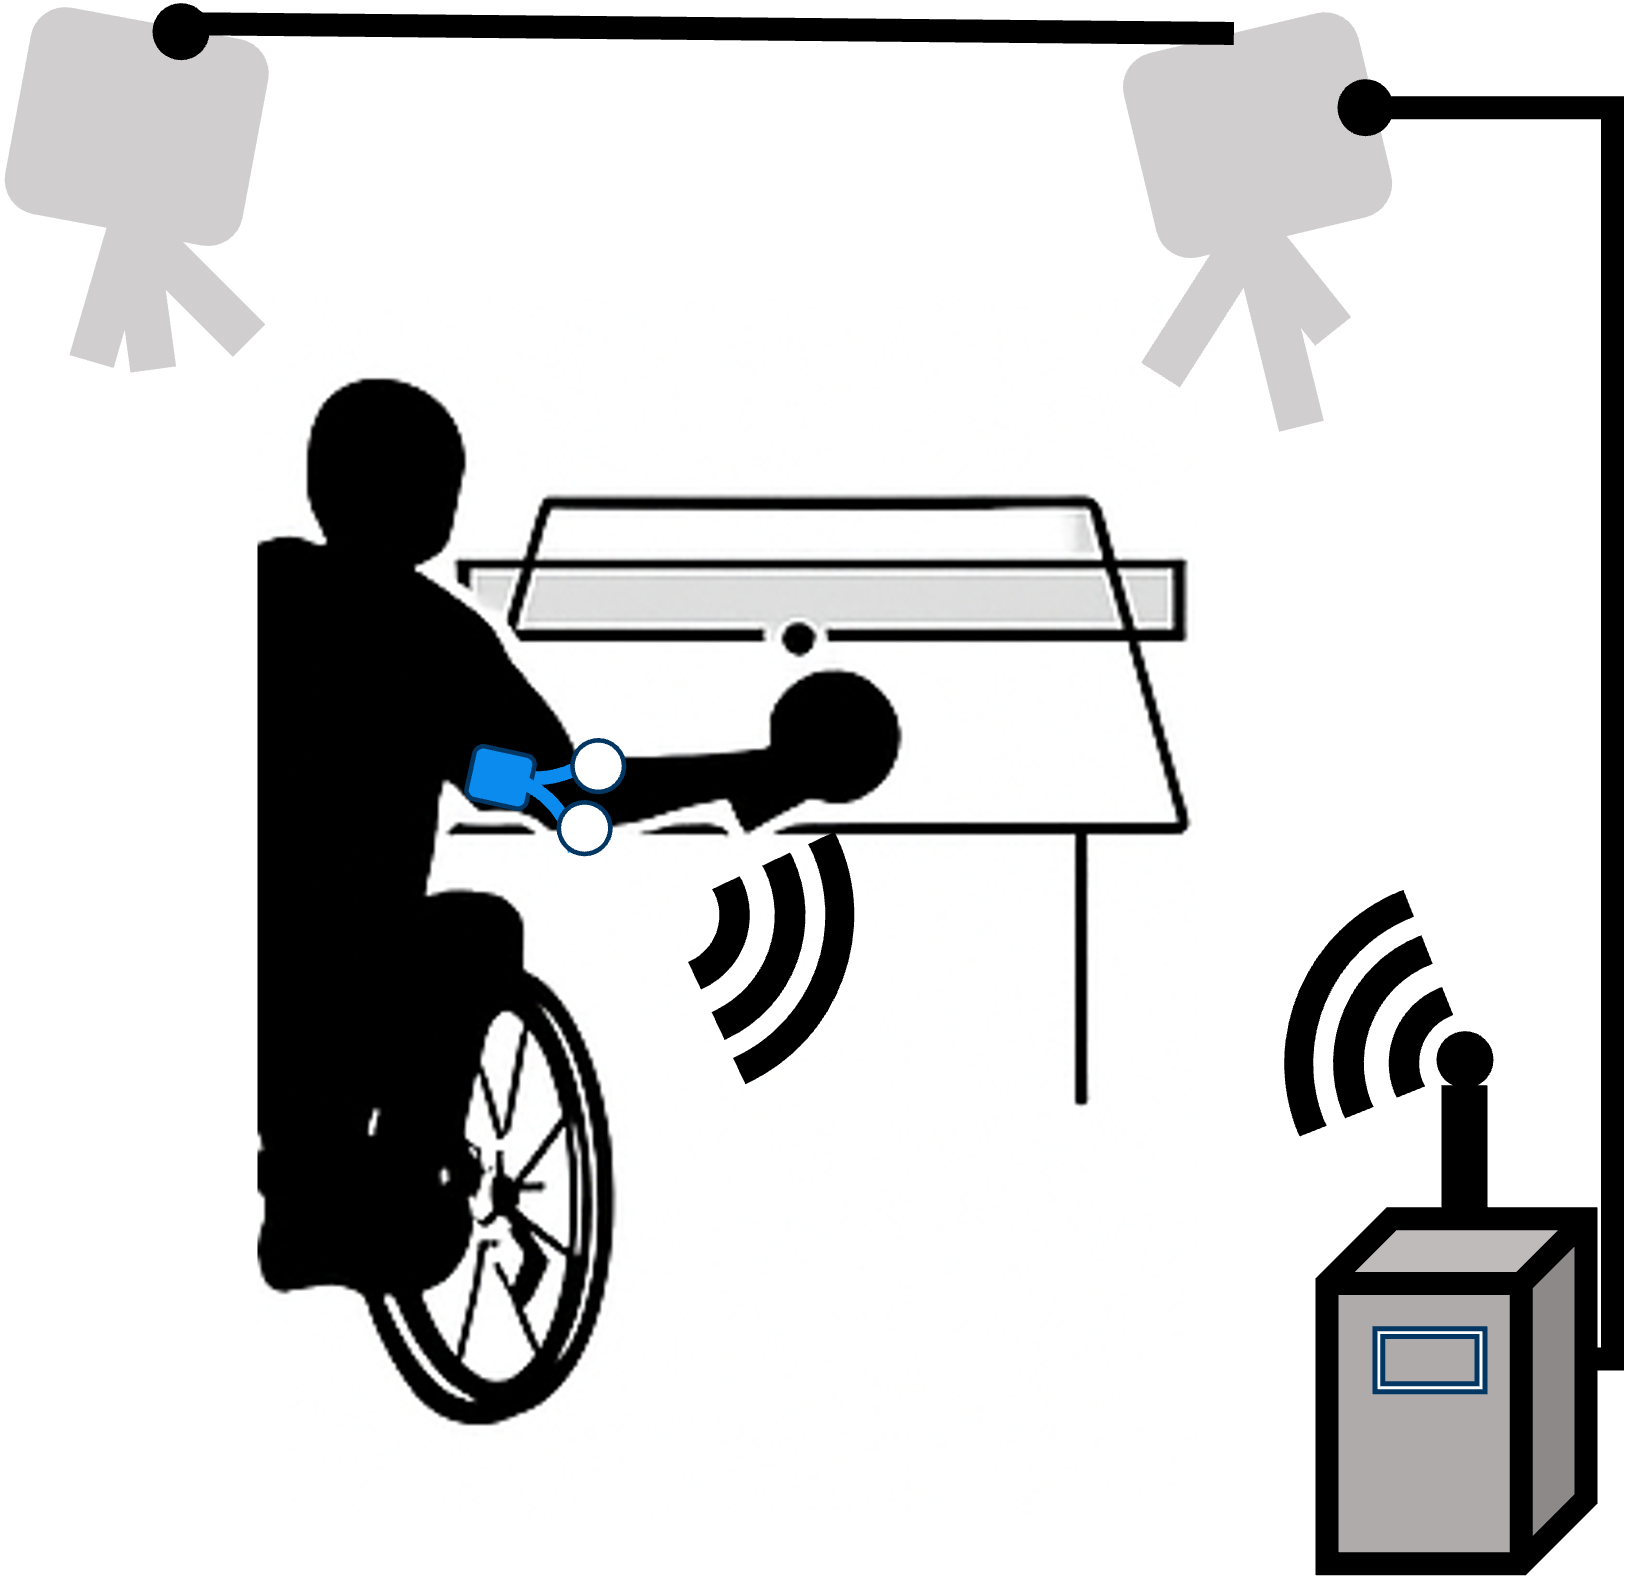
\includegraphics[keepaspectratio,width=0.8\linewidth]{chap2/exp_setup.png}%論文中の実験環境図
\caption{計測システムの概要と実験環境}
\label{fig:experimental_setup}
\end{figure}

\subsection{階層的解析プロセス}
取得したデータに対し，決定論的モデルに基づき以下の3段階で解析を行った．

\begin{enumerate}
\item\textbf{パフォーマンスの定量化}:
高速度カメラ映像からインパクト後のボール軌道を算出し，ターゲット中心からのユークリッド距離$D$を打球精度の指標（目的変数）とした．また，誤差$D$に基づき，高精度群（Good）と低精度群（Bad）への分類を行った．

\item\textbf{ラケット挙動解析（第1階層）}:
インパクト時のラケットの位置・速度・角度など計12個の物理パラメータを算出した．これらを入力とし，打球精度クラスを予測する機械学習モデル（ランダムフォレスト等）を構築した．さらに，PermutationFeatureImportance(PFI)を用いて，予測精度に寄与する重要変数を特定した．

\item\textbf{身体動作・筋活動解析（第2・3階層）}:
特定された重要なラケット変数を目的変数とし，ステップワイズ法を用いた重回帰分析により，ラケット挙動に影響を与える関節運動（肩・肘・体幹など）を特定した．最後に，それらの関節運動に関連する筋群の活動電位（RMS）を比較し，精度の良し悪しを分ける筋活動パターンを抽出した．
\end{enumerate}

\section{結果と考察}

\subsection{打球精度の決定要因：ラケット挙動}
機械学習モデルによる重要度分析の結果，打球精度を決定づける支配的なラケット要因として以下の3つが特定された．
\begin{itemize}
\item\textbf{ラケット面角度($\phi^{\text{Vert}}$)}:被せ角の安定性が最も重要であり，面が開きすぎるとオーバーミス，閉じすぎるとネットミスに直結した．
\item\textbf{水平打ち出し角($\theta^{\text{Horz}}$)}:ターゲット方向へ正確に打ち出すための角度制御．
\item\textbf{長軸方向の打点位置($d_{\text{Long}}$)}:手元ではなく，ラケット先端（スイートスポット）で捉えることの重要性が示された．
\end{itemize}
回帰分析の結果，これらの変数は決定係数$R^2>0.6$で身体動作によって説明可能であることが示された．

\subsection{ラケット挙動を生成する身体動作と筋活動}
特定されたラケット要因に対し，Good群とBad群の動作・筋活動を比較解析した結果，以下の知見が得られた．

\subsubsection{運動連鎖とブレーキング動作}
精度の高い打球（Good群）では，運動連鎖（KinematicChain）の原則通り，近位セグメントから遠位セグメントへと順次エネルギーが伝達されていた．
図\ref{fig:kinematic_chain}に示すように，インパクト直前において，まず体幹回旋と肩関節屈曲が減速（ブレーキング）し，そのエネルギーが肘の伸展および前腕の運動へと転移していることが確認された．
Putnamらが提唱するように\cite{putnamSequentialMotionsBody1993}，近位の減速が遠位の加速を生み出し，ラケットヘッドの走りと操作性を向上させている．

\begin{figure}[tb]
\centering
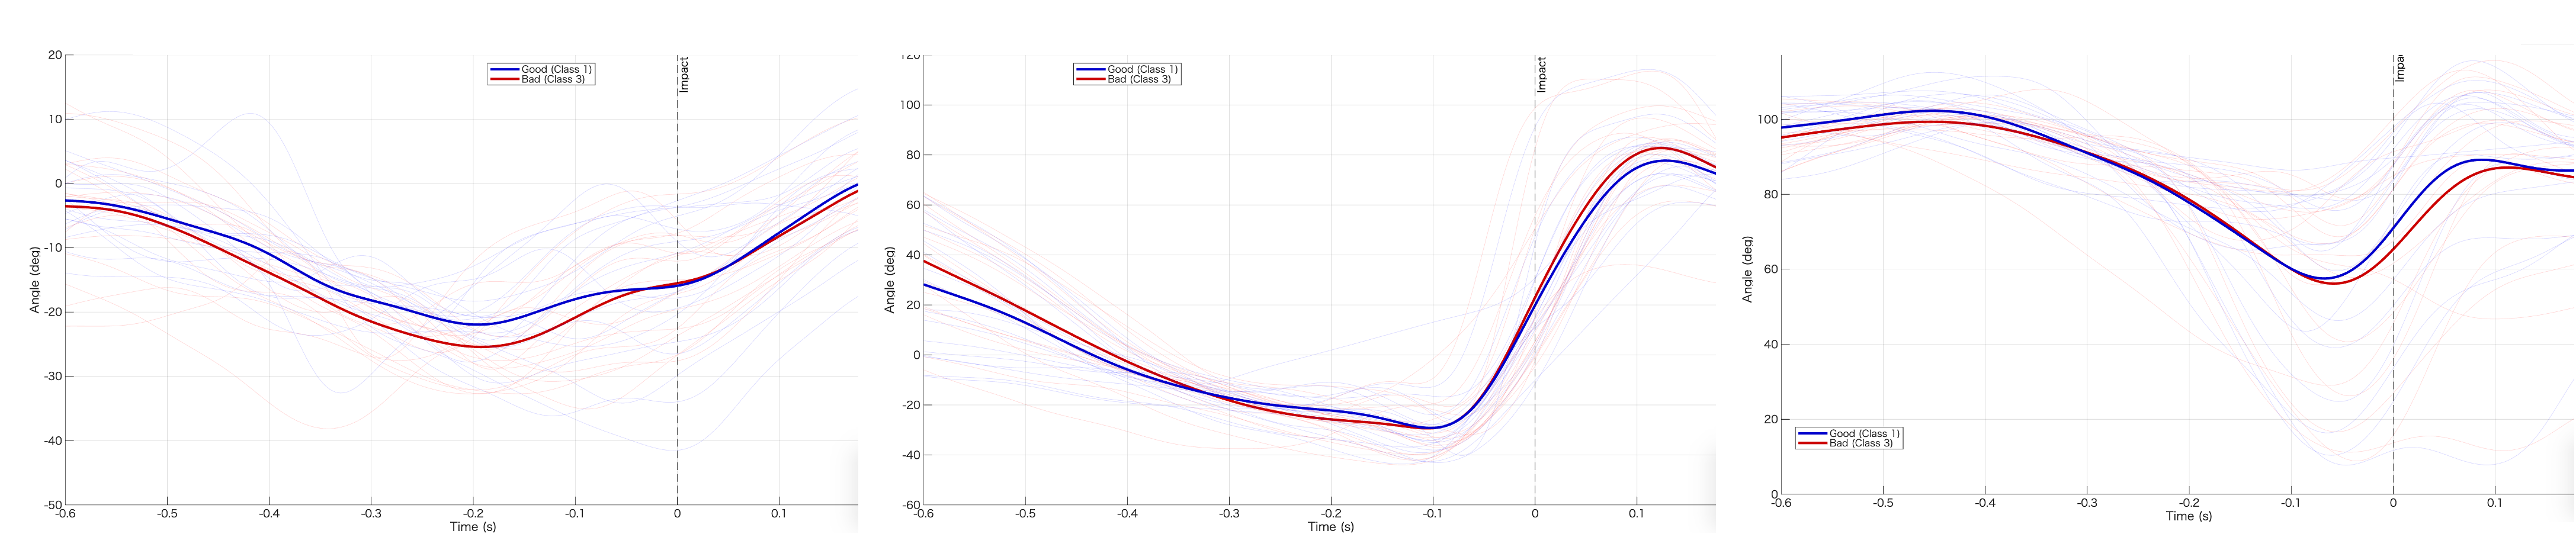
\includegraphics[keepaspectratio,width=0.9\linewidth]{chap3/kinematic_chain.png}%論文中の角速度波形等の図
\caption{Good群における角速度波形の推移．近位（肩）の減速に伴い遠位（肘・ラケット）が加速している．}
\label{fig:kinematic_chain}
\end{figure}

\subsubsection{筋活動による動作制御}
この運動連鎖を筋活動の観点から検証した．
Good群では，フォワードスイング初期に主動筋である三角筋前部や大胸筋が強く活動するが，インパクト直前には活動が急速に低下（弛緩）していた．これにより肩関節の減速がスムーズに行われ，遠位へのエネルギー転移が実現されていた．
一方，Bad群では，インパクト時まで三角筋前部等の過剰な共収縮（Co-contraction）が見られた．
これは，心理的な力みや姿勢制御の不備により，腕全体を固めて「押し出す」ようなスイングになっていることを示唆している．
この「押し出し動作」は，ラケット先端速度の低下を招くだけでなく，ラケット面角度の微調整を困難にし，結果として打球精度の低下（特に打点位置のばらつきや面角度の不安定化）を引き起こしていると結論づけられる．

\subsubsection{体幹機能の影響}
また，水平打ち出し角のばらつきには，体幹回旋のタイミングが大きく関与していた．
遠位打球へのリカバリーにおいて，体幹の回旋が遅れた場合，手先だけの操作で打球方向を修正しようとする代償動作が発生し，これがインパクト時のラケット角度の不安定性を増大させていた．
クラス4の選手にとって，残存する体幹機能を最大限活用し，早期に身体の向きを作るポジショニングが，上肢の自由度を確保するために重要であることが示唆された．

\section{結論}
本研究では，車椅子卓球選手の打球精度を決定づける要因を，決定論的モデルに基づいた階層的解析によって明らかにした．
主な知見は以下の通りである．

\begin{enumerate}
\item打球精度は「ラケット面角度」「水平打ち出し角」「ラケット先端での打撃」に強く依存する．
\item高精度な打球の実現には，運動連鎖に基づく近位から遠位へのエネルギー伝達が不可欠である．
\item筋活動レベルでは，インパクトに向けた近位筋（三角筋等）の適切な弛緩（ブレーキング）が，ラケット操作の自由度と安定性を高める鍵となる．
\item不適切な筋の共収縮や体幹回旋の遅れが，ラケット挙動の不安定化を招く主要因である．
\end{enumerate}

本手法は，単なる動作観察では捉えきれない，パフォーマンスに直結する内部的な身体制御メカニズムを可視化するものである．
これにより，選手の障害特性や個別の筋活動パターンに応じた，科学的根拠に基づくコーチングへの応用が期待される．

\bibliographystyle{pesummary}
\bibliography{sections/reference,sections/reference_web}
\end{document}
